\documentclass[sigconf, timestamp-false, anonymous=true]{acmart}

\usepackage{listings}
\usepackage{multirow}
\usepackage{graphicx}
\usepackage{subcaption}
\usepackage{hyperref}
\usepackage{fancybox}

%% Rights management information.  This information is sent to you
%% when you complete the rights form.  These commands have SAMPLE
%% values in them; it is your responsibility as an author to replace
%% the commands and values with those provided to you when you
%% complete the rights form.
\setcopyright{none}

\acmConference[ESEC/FSE '20]{ESEC/FSE '20: ACM Joint European Software Engineering Conference and Symposium 
on the Foundations of Software Engineering}{November 8-13, 2020}{Sacramento, CA, USA}
\acmYear{2020}

\newcommand\todo[1]{\textcolor{red}{#1}}

%%
%% Submission ID.
%% Use this when submitting an article to a sponsored event. You'll
%% receive a unique submission ID from the organizers
%% of the event, and this ID should be used as the parameter to this command.
%%\acmSubmissionID{123-A56-BU3}

%%
%% The majority of ACM publications use numbered citations and
%% references.  The command \citestyle{authoryear} switches to the
%% "author year" style.

%%
%% end of the preamble, start of the body of the document source.
\begin{document}

\title{A Study of Multi-Edit Bug Patches}

%add authors & shortauthors if we are lucky :)

\begin{abstract}
  \todo{note that this is probably full of falsehoods, I'm just thinking by
    typing.} Automatic program repair is a promising approach for reducing the
    cost of quality assurance practices and faulty software. To date, most
    techniques proposed for test-driven automatic repair have succeeded
    primarily on bugs that benefit from short, single-edit patches. Techniques
    that succeed on multi-edit bugs often do so by patching them in an
    alternative, single-edit way, or by targeting particular multi-edit bug
    patterns. Empirical studies of real-world similarly tend to focus on the
    patterns exhibited by single-edit bugs, and have not examined repairability
    of multi-edit bugs in detail. We present a comprehensive empirical analysis
    of multi-edit bugs in open source Java programs, focusing on static and
    dynamic properties that define the repair search space for a given bug (and
    thus, in turn, the challenges that apply to automatically addressing them).
    This analysis focuses on the key challenges of the dynamic program repair
    problem: the \emph{mutations and fix code} used to repair multi-edit bugs;
    the \emph{fault locations} and their relationships; and the \emph{objective
      function}, and in particular how and to what degree test cases can be used
    (or not) to identify partial repairs. We identify key takeaways and
    challenges, with implications for future work in expressive, multi-chunk bug
    repair.
\end{abstract}

%%
%% The code below is generated by the tool at http://dl.acm.org/ccs.cfm.
%% Please copy and paste the code instead of the example below.
\begin{CCSXML}
<ccs2012>
<concept>
<concept_id>10011007.10011074.10011099.10011102</concept_id>
<concept_desc>Software and its engineering~Software defect analysis</concept_desc>
<concept_significance>500</concept_significance>
</concept>
<concept>
<concept_id>10011007.10011074.10011784</concept_id>
<concept_desc>Software and its engineering~Search-based software engineering</concept_desc>
<concept_significance>500</concept_significance>
</concept>
</ccs2012>
\end{CCSXML}

\ccsdesc[500]{Software and its engineering~Software defect analysis}
\ccsdesc[500]{Software and its engineering~Search-based software engineering}

\keywords{software bugs, program repair}

\maketitle


\newcommand{\rqorinsight}[2]{
  \setlength{\fboxsep}{0.8em}
  \vspace{0.5em}
  \begin{center}
  \Ovalbox{\begin{minipage}{0.9\linewidth}
    \textbf{Research Question:} #1
    \end{minipage}}
  \end{center}
  \vspace{0.5em}}

\section{Introduction}

Buggy software has a significant cost in terms of both social impact~\cite{tricentis} 
and developer effort~\cite{cambridge-study}. This
motivates significant research in techniques to automatically find and fix
them~\cite{whatever}, with the ultimate goal of reducing Quality Assurance costs
while improving software quality. 

A significant class of program repair techniques in both
research~\cite{genprog,angelix,Le17, Xuan17} and practice~\cite{sapfix} use test cases to guide
patch construction, typically by following what's known as a
generate-and-validate paradigm. At a high level, these techniques use test cases
to localize a defect --- identified by at least one failing test --- to a set of
likely-suspicious program locations. Then, they use a variety of techniques to
construct (or \emph{generate}) patch candidates for the bug in question,
checking each to see (or \emph{validate}) if any of them cause the program to
pass all of the provided test cases.  
%
Patches are constructed in a variety of ways, ranging from heuristic, syntactic
program manipulation~\cite{par,genprog,rsrepair,ae,prophet,hdrepair}, to specially adapted program
synthesis techniques~\cite{Konighofer11,Konighofer12,semfix,DeMarco14,angelix}. These techniques have successfully
repaired real, meaningful defects in large, complex
programs~\cite{angelix,genprog-eight-dollars,prophet,sapfix}.

Practically speaking, these techniques are typically limited in the types and
variety of defects they can repair~\cite{for,example}. Some of this limitation
is by design. Some techniques specifically target certain classes of
bugs~\cite{nopol,sapfix}, and it has been argued that doing so is necessary for
repair to reach true practical applicability~\cite{maybe}. Fundamentally, the
vast majority of program repair techniques can only produce single-edit repairs,
often by design~\cite{rsrepair, ae, hdrepair}. \todo{more recent citations?}
Even those that can in principle produce multi-edit bugs typically
don't~\cite{poor,genprog}.

This leaves a large proportion of real-world bugs unrepairable by modern
research techniques in program repair.  Over half of the bugs in popular bug
benchmark Defects4J are patched by humans using multi-part
patches~\cite{d4j-dissection}. Approximately 70\% of buggy source files in a
large study of bugs in Apache projects required two or more edit
actions~\cite{zhong2015}.

A key factor or tension in how these techniques are constructed is in their
management of the trivially-infinite search space of possible patches for a
given bug, while constructing patches in which a user can have confidence of
their quality or correctness.  This space has been parameterized~\cite{refs}
along several axes: (1) the \emph{fault space}, or the potential locations that
may be changed, (2) the \emph{mutation space}, or the possible modifications
that may be tried at a location, and (3) \emph{fix code space}, or the code that may
be instantiated as part of a mutation (e.g., if the mutation seeks to
\emph{insert} code, the fix code is the code that is inserted).  Many dynamic
repair techniques can be compared or described in terms of their choices along
each of these axes; the ways each technique constructs and then traverses the
space has first-order implications for scalability, and for the type and quality
of patches produced.  This has been studied many ways~\cite{examples}.

Multi-edit repair poses distinct challenges for each of these axes for repair.  
Spectrum-based fault localization, the most
prevalent class of fault localization techniques used in program repair, does
not specifically identify sets of locations that might be related or repaired
together; indeed, the evaluation of most fault localization
techniques typicaly assumes that a bug is localized if any one buggy line is
identified~\cite{fl-survey-wong}.  Researchers have observed that some bugs are
repaired in multiple locations using very similar
code~\cite{saha2019harnessing,jiang2019cmsuggester}, informing novel techniques
that constrain the \emph{fix space} of possible multi-edit repairs accordingly.
One key question for applicability of these types of techniques is how prevalent
such bugs are, and how often multi-edit bugs instead require multiple
coordinating (but ultimately different) edits or pieces of fix code.  Over 50\% of the fixes in four 
Apache projects involve two or more entities -- i.e., a Java class, method, or field -- and 66\%-76\% of 
those multi-entity fixes involved syntactic dependencies.~\cite{wang2018}. 
Test cases are used to evaluate candidate repairs in virtually all dynamic
generate-and-validate repair techniques, but, anecdotally, may not be effective
at identifying partial repairs in a multi-edit
context~\cite{fitness10,maybeeric}.  
Although multi-edit repair has been discussed in the context of other analyses
that study bug fix characteristics in general~\cite{examples} as well as for
repair applicability specifically~\cite{moar,examples}, to the best of our
knowledge there has been no significant previous study of the characteristics of
multi-edit repairs in terms of their implications for repairability or, more
broadly, program repair.  

In this paper, we present a systematic study of real-world multi-edit bugs,
looking specifically at their characteristics with respect to the problem of the
automatic repair search space.  
We study the bugs curated in two
real-world datasets that support program repair research: Defects4J~\cite{defects4j}
and BEARS~\cite{bears}, in total, 576 bugs in 40 projects. 
More than half of these bugs were repaired by a
human developer using a multi-chunk repair (as we define in
Section~\ref{sec:background}).  We look at characteristics along each of the
relevant axes of the program repair search problem: fault locations, mutation
operators, fix code, and evaluation (or fitness or objective) using test cases.  Our 
contributions are
as follows:

\begin{itemize}
\item An analysis of multi-edit bug patches in Defects4J and Bears.
\item A study characterizing the ways that failing tests cover faulty locations as a means of 
testing whether the underlying hypothesis in current fault localization techniques still hold 
in multi-edit bugs. We find that 58\% of 
bugs with multi-edit patches and multiple failing tests have faulty locations that are not 
covered by all failing tests, thus the underlying assumptions do not necessarily hold.
\item A study characterizing fix code.  We find that half of 
bug patches contain dependent edits and \todo{N\%} contain 
code clones.
\item A new fitness function that measures patch quality using the number of 
	passing and failing assertions within test cases.
\item study of test cases as a means to evaluation partial and full
  multi-site repairs.  We find that there are significant amount of edit chunks that
  is not captured by test cases, as a third of Defects4j multi-chunk bugs and over a half of 
  Bears multi-chunk bugs do not require all edit chunks in their provided human patches to
  pass all test cases. Other than that, we found that, under highest granularity (assertion level), test case
  based validation methods can positively identify over 40\% of partial repairs, 
  while less than 40\% partial repairs are neutral in test cases and less than 20\% are identified
  negatively. Moreover, we found that higher granularity will increase the number of
  positively identified partial repairs, but it will also increase the number of negatively 
  identified partial repairs, and the amount of increase/decrease may vary between
  datasets.
\item  study of code clones. We find that over 30\% multi-chunk bugs
  have almost same edits applied to different locations. Moreover, bugs that have 
  "disjoint" coverage result tend to be much more likely (19 out of 23) to have
  code clones.
\item \todo{A set of recommendations?}
\end{itemize}

\todo{This paragraph is a lie and some people hate them so maybe we'll cut it,
  it just feels comforting to me to write them as I'm working on a paper draft...}
The rest of this paper is organized as follows.  We provide background on
generate-and-validate program repair, with a focus on the key parameters of the
program repair search problem, in Section~\ref{sec:background}.  We describe the results of our analysis in
Section~\ref{sec:results}, with discussion of implications as well as
limitations in Section~\ref{sec:discussion}.  Related work is discussed in
Section~\ref{sec:related}; Section~\ref{conclusions} concludes.

\section{Key Concepts and Research Questions}
\label{sec:background}

\paragraph{Search spaces in automatic program repair.} Automatic program repair (APR) techniques aim to find patches for bugs in
programs.  We restrict attention to dynamic or test-case guided program repair,
which describes the majority of research advancements over the past ten years.
Such techniques take as input a program and a set of test cases that serve as
the oracle for program correctness.  At least one of those tests should be
failing, corresponding to the bug to be repaired.  

At a high level, any APR technique aims to solve a search or optimization
problem, seeking a set of edits (or patch) to the program that will lead it to
pass all of the provided tests.  Although The repair search is classically defined along
the following axes:
\begin{itemize}
\item \emph{Fault space.} The first problem in fixing a bug concerns
  \emph{where} in the code modifications should be applied. All dynamic repair
  techniques begin by using the provided test cases as input to a fault
  localization technique. Such techniques identify (and typically score)
  suspicious code based on which test cases execute which pieces of code.
  Although the particulars of the fault localization employed can vary, most APR
  use some variant of spectrum-based fault localization (SBFL)~\cite{refs} in
  this first step. The resulting computation defines the fault space, or the
  candidate locations or code entities considered for repair. This first step is
  key to reducing the search space.

\item \emph{Mutation space.} The mutation space is the set of applicable 
modifications at a program location. Examples include GenProg's append, 
replace, and delete operators over statements~\cite{genprog-operators} and 
Nopol's condition replacement over if-statements and missing precondition 
addition over non-branch and non-loop statements~\cite{Xuan17}.
A larger mutation space generates 
a richer search space with potentially more repairs, but
the resulting combinatorial growth of the search space can also hinder 
the search process~\cite{long-search-spaces}.

\item \emph{Fix code.}

\item \emph{Objective.} 

\end{itemize}



\paragraph{Edit granularity in bug-fixing patches.}  Developer patches for
program bugs naturally vary in length and complexity.  Estimates range from
\todo{FIXME} to \todo{FIXME}\% of bugs are repaired using fewer than
\todo{FIXME} lines of code.  \todo{rephrpase/repeat stuff in intro about
  studies/prevalence of multi-edit bugs, but expand the rephrase of the results
  in that prior work to contrast with incidence of single-edit bugs.}  

There are indeed several plausible definitions of multi- vs. single-edit bugs,
with implications for how they are studied.  We consider edits at the granularity 
of lines and of chunks. We define a line edit as an added, removed, or modified 
line. We define a chunk as a continuous sequence of line edits, with the exception 
that if one chunk adds a \texttt{\{} whose corresponding \texttt{\}} is in a different chunk, 
then we merge the two chunks together. 
We ignore changes to comments, whitespace, or import statements.

Alternative definitions may have bearing on our results.  We argue that this
definition is natural for the purposes of our study, which focuses in particular
on understanding larger bugs---especially multi-chunk bugs---for the purposes of 
adapting, extending, or applying new program repair techniques to address them. 
\todo{A couple more sentences re: why this is reasonable. Might be solved by 
pointing to low rates of repair for multi-chunk bugs.}

\paragraph{Research questions.}  The parameterization of the program repair
search problems into multiple subspaces informs our empirical study of those
spaces for the purposes of understanding multi-edit repair.  We address the
following research questions:

\begin{enumerate}
\item \emph{RQ1: How prevalent are multiedit human patches are in Defects4J and Bears?}
\item \emph{RQ2: Do failing tests cover different portions of the fault?}
\item \emph{RQ3: How prevalent are dependencies between edited code?}
\item \emph{RQ4: How often do code clones occur in multi-chunk bugs? Are existence of 
code clones in human patch correlated with specific patterns of fault localization?}
\item \emph{RQ5: Do test cases fully capture the effects of multiple edits?}
\item \emph{RQ6: How well do test case based validation methods identify partial repairs?}



\end{enumerate}

\section{Dataset Characteristics}
\label{sec:data-rq1}

\begin{table}
\begin{center}
\begin{tabular}{l | rrr}
\toprule
\multicolumn{4}{c}{\textbf{Defects4J}} \\
\midrule
Project & Bugs & Src (kloc) & Test (kloc) \\
\midrule
JFreeChart  & 26 & 193.3 & 74.6 \\
Closure compiler & 133 & 150.6 & 112.6 \\
Apache commons-lang & 65 & 57.8 & 47.4 \\
Apache commons-math & 106 & 45.0 & 41.5 \\
Mockito & 38 & 23.0 & 28.5 \\
Joda-Time & 27 & 82.9 & 70.4 \\
\midrule
\multicolumn{4}{c}{\textbf{Bears (single-module)}} \\
\midrule
FasterXML-jackson-databind & 26 & 95.7 & 53.6 \\
INRIA-Spoon & 62 & 66.2 & 30.8 \\
spring-data-commons & 15 & 45.8 & 28.8 \\
traccar-traccar & 42 & 47.9 & 8.6 \\
30 other projects & 62 & - & -\\
\bottomrule
\end{tabular}
\end{center}
\caption{\label{tab:data} Characteristics of the Defects4J (top) and Bears (bottom) datasets.}
\end{table}

\todo{I think we should add a column to the datasets indicating how many of each are multi-test, as well} 

\paragraph{Datasets}  Our study requires a dataset of indicative, real-world,
multi-edit defects.  We study both the defects in Defects4J
Defects4J~\cite{defects4j} and Bears~\cite{bears}.  Table~\ref{tab:data}
summarizes these datasets, both of which
consist of historical
bugs found in real world software projects. Defects4J contains 395 bugs from 
six Java software projects, and is currently very popular dataset for evaluating 
program repair tools that target Java~\cite{durieux-repair-them-all}.
However, there is a risk associated with any such dataset that tools may overfit
to the defects in question, and there is evidence that this situation applies to
program repair and Defects4j~\cite{durieux-repair-them-all}. 
We thus also study bugs from Bears~\cite{bears}, 
a set of Java bugs derived from failed Travis-CI builds of GitHub
projects. 
Bears offers 251 bugs from 72 software projects, providing a greater diversity of 
projects compared to Defects4J. 
Several projects in Bears, however, are structured as multi-module projects, 
which are not currently compatible with our automation tools.
We thus limit our analysis of Bears to 181 bugs from 30 single-module projects.
We intend to address the remaining multi-module software projects in future work.

\todo{Consider adding a column to the dataset table above with ``subset
  considered'' for the defects; is this worth doing?  How many bugs do we
  exclude? Do we include Closure?}

\begin{table}
{\begin{center}
	\begin{tabular}{l | rr | rr | rr}
		\toprule
		\multicolumn{7}{c}{\textbf{Line edit granularity}} \\
		\midrule
		Dataset & \multicolumn{2}{c}{Single line} & \multicolumn{2}{c}{Multi-line} & \multicolumn{2}{c}{Total} \\
		\midrule
		Defects4J & 92 & 23\% & 303 & 77\% & 395 & 100\%\\
		Bears & 27 & 15\% & 154 & 85\% & 181 & 100\%\\ 
		Combined & 119 & 21\% & 457 & 79\% & 576 & 100\% \\ 
		\midrule
		\multicolumn{7}{c}{\textbf{Chunk edit granularity}} \\
		\midrule
		Dataset & \multicolumn{2}{c}{Single chunk} & \multicolumn{2}{c}{Multi-chunk} & \multicolumn{2}{c}{Total} \\
		\midrule
		Defects4J & 211 & 53\% & 184 & 47\% & 395 & 100\%\\
		Bears & 72 & 40\% & 109 & 60\% & 181 & 100\%\\
		Combined & 283 & 49\% & 293 & 51\% & 576 & 100\%\\
		\bottomrule
	\end{tabular}
 \end{center}
}
	\caption{Frequencies and percentages of bugs with multi-edit patches
	based on the edit granularities defined in Section~\ref{sec:background}.
	Multi-line patches comprise a large majority of patches, and multi-chunk 
	patches comprise a majority or a large minority of patches in both datasets.}
	\label{tab:multiedit-frequencies}
\end{table}


\todo{Please combine table 1 and table 2 as suggested over slack}

\subsection{Multi-edit Prevalence}
\rqorinsight{RQ1: How prevalent are multi-edit human patches are in Defects4J and Bears?}

We start our analysis of multi-edit patches by asking how many such patches 
exist in our benchmarks. We analyze edits at line and chunk granularities,
which we defined in Section~\ref{sec:background}.

\paragraph{Results} 
Table~\ref{tab:multiedit-frequencies} lists the number and percentages of
multi-line and multi-chunk patches in Defects4J and Bears. 
Multi-line patches comprise a large majority of patches across both datasets, 
while multi-chunk patches comprise over half of Bears and almost half of Defects4J.
At both levels of edit granularity, Bears contains a greater proportion of 
multi-edit patches compared to Defects4J.

\todo{Maybe add some data to show repair rates of multi-line \& multi-chunk bugs}

\todo{CLG says: ...I honestly don't understand the ``frequencies'' table or the
  2--3 sentences above. And: What is the interpretation?
  Why do I care?}


\section{Fault localization}

%% what are the claims, what are we studying, why are we studying it


Spectrum-based fault localization (SBFL) is the most commonly studied, as well as the most 
effective~\cite{zou2019empirical}, fault localization technique. It is a key
first step to characterizing the \emph{fault space} in automatic program repair,
narrowing the search space to a portion of the program more likely (based on
test case behavior) to correspond to the fault.  

\paragraph{SBFL Basics.} \todo{Serena, please add an explanation of how SBFL
  works; it's key to understanding the underlying assumption.  This should
  include references as appropriate.}

Given these basics, fundamentally, a core
assumption underlying SBFL is that \emph{failing tests execute buggy portions of 
the code relatively more often than passing tests.} Thus, if all failing tests execute a 
particular line of code, then that line of code is scored as more suspicious.
This assumption is well-suited to single edit repair. Indeed, the evaluation
of most SBFL techniques asks exactly the question of interest when considering a
technique's suitability for single-edit repair: how often does a given technique
correctly, highly rank individual buggy lines of code? 

Such evaluations, by and large, do not consider the implications of
suspeciousness scoring in a multi-edit repair context.  Instead, evaluations
typically consider a technique ``successful'' if it identifies \emph{any} of a
set of changed lines as highly-ranked or likely-suspicious.  While appropriate
for the question being asked in such evaluations, this does not address
suitability for multi-line program repair.  Identifying one of several buggy
locations is generally inadequate in a context where multiple locations must be
modified.  

Thus, in this research question, we investigate how well the SBFL assumption
applies to tests that identify multi-line bugs. We focus especially on
multi-line bugs that are associated with multiple tests; \todo{short explanation
  of the intuition why. This is a placeholder, I'm a bit tired and so this
  succinct explanation is escaping me.} If multiple tests all cover the multiple
modified locations well, then SBFL's core assumption holds and multi-edit repair
can expect to effectively make use of the off-the-shelf ranking these techniques
currently provide (indeed, this has been tried~\cite{angelix}). If not---that
is, if multiple tests exercise \emph{different} portions of the buggy
code---SBFL off-the-shelf will by definition be less effective in guiding APR to
correctly modifying multiple buggy locations at once.

Therefore, for multi-edit bugs with multiple identifying failing tests, do the 
different failing tests cover exactly the same patch locations, exactly 
disjoint path locations, or some combination?


\rqorinsight[2]{How well do multiple tests cover the multiple locations
  implicated in multi-edit bugs?}

\paragraph{Methodology}

Between both datasets, there are 60 total bugs that are both multi-edit and 
multi-test -- 45 in Defects4J and 15 in Bears. For each of these bugs, we used 
Jacoco to determine which of the chunks in the human patch were executed by each failing test. Using 
this coverage data, we categorized the bug as one of 
three coverage patterns: \textit{disjoint} for bugs in which no chunk is covered by all failing tests, 
\textit{same} for bugs in which all 
tests cover the exact same chunks of the patch, and \textit{overlap} for all 
other bugs, where some chunks are covered by all failing tests, but some chunks are only covered by a 
subset of failing tests.

\paragraph{Results}
The overall distribution is seen in Figure \ref{fig:coverage-all}. Over a third 
of the bugs were classified as disjoint, indicating that for a significant 
portion of bugs, the failing tests do not all execute any portion of the faulty 
code. In addition, another 22\% were classified as overlap. Thus, over half of 
the bugs that were both multi-edit and multi-test contained chunks that were 
not executed by all failing test cases.
2

\begin{figure}
	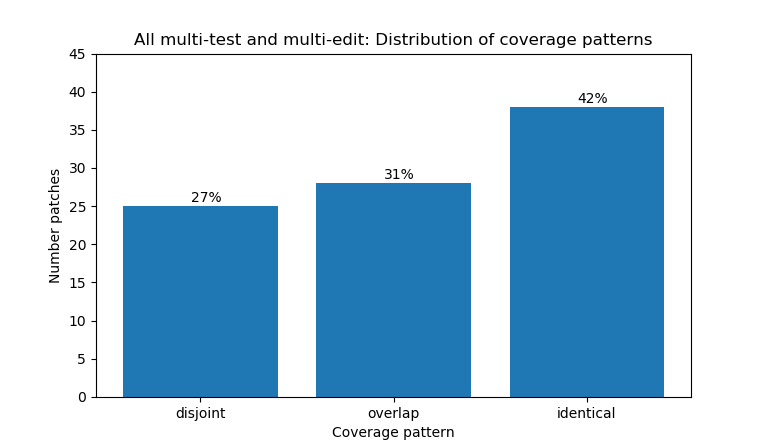
\includegraphics[width=\linewidth]{img/coverage-all.png}
	\caption{Distribution of coverage patterns for all multi-test and 
	multi-edit bugs in Bears and Defects4J. In all, 38\% of bugs were classified as disjoint, 40\% were 
	classified as same, and 22\% were classified as overlap.}
	\label{fig:coverage-all}
\end{figure}

SBFL assumes that faulty locations are executed more often by identifying 
or failing test cases and is not designed to find faults like these. Since SBFL 
is the most common fault localization technique in APR, most APR techniques 
are not well suited to fix a majority of these multi-edit and multi-test 
bugs.

If we divide distribution by dataset, we can see even more interesting 
behavior. Figure \ref{fig:coverage-datasets} shows the Defects4J dataset and 
the Bears dataset have very different distributions with respect to the 
disjoint and same categories -- in Defects4J, 47\% of bugs are disjoint and 
31\% are same, whereas in Bears, the proportions are 13\% disjoint and 67\% 
same. We hypothesize that this may be due to differences in how the two 
datasets were minimized, since Defects4J is a dataset of minimized and curated 
bugs while the bugs in Bears are taken scraped directly from the commits.


\begin{figure}
	\begin{subfigure}{\linewidth}
		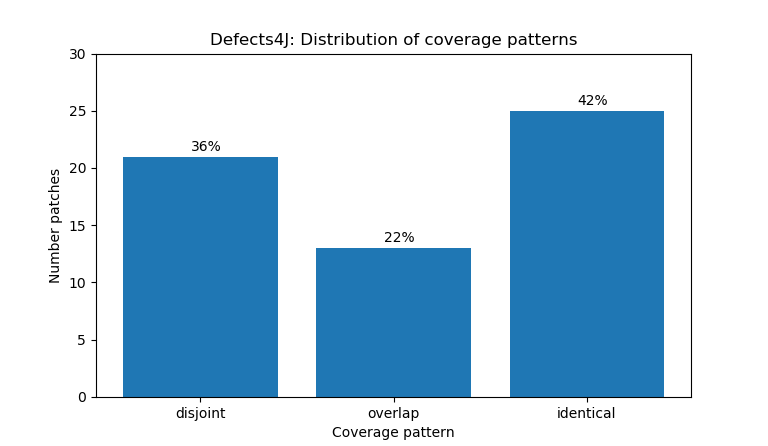
\includegraphics[width=\linewidth]{img/coverage-d4j.png}
		\caption{Distribution of coverage patterns for Defects4J. 47\% disjoint, 31\% same, and 22\% 
		overlap.}
	\end{subfigure}
	\begin{subfigure}{\linewidth}
		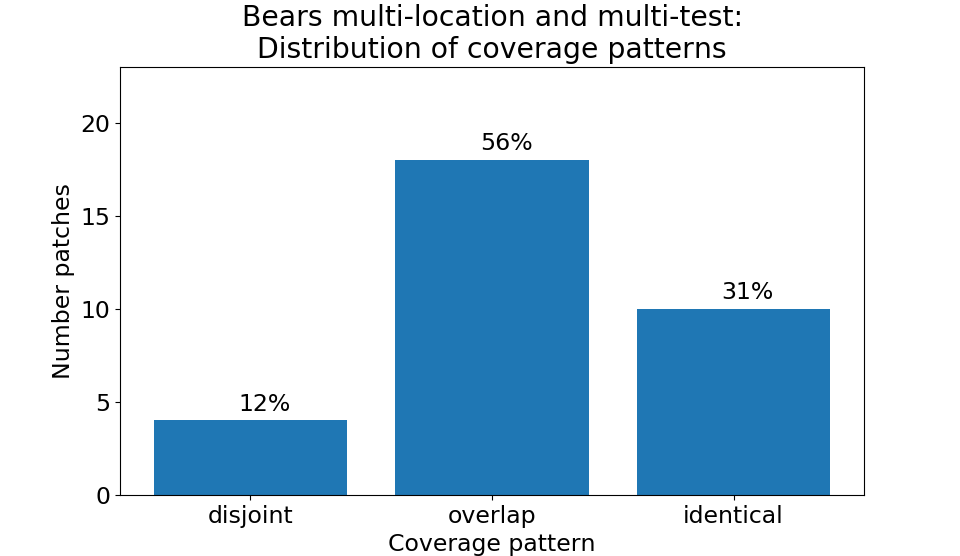
\includegraphics[width=\linewidth]{img/coverage-bears.png}
		\caption{Distribution of coverage patterns for Defects4J. 13\% disjoint, 67\% same, and 20\% 
		overlap.}
	\end{subfigure}
	\caption{Distribution of coverage patterns divided by dataset.}
	\label{fig:coverage-datasets}
\end{figure}


%\section{Symptoms}

We want to study symptoms in the context of fault localization. We define symptoms as the output given in failing test cases. In Java, most of these symptoms will be exceptions and their accompanying error message. Since most program repair is based off of failing tests, we want to see if those symptoms exhibited in those tests can correlate to type of repair.

For this paper, we specifically wanted to look at whether symptoms correlated with whether a bug could be fixed in a single location or multiple locations. If we can classify which bugs are single edit or multi edit, we can choose fault localization or patch generation techniques that are more suited.

We looked at all symptoms for all bugs in Defects4J and Bears, and categorized them based on whether they were one of the identified multi-chunk bugs or not. Then we fit the data to a linear regression model to see if there were statistically significant differences between the type of symptoms for multi edit and single edit bugs.

In order to find statistical significance, we needed to categorize the symptoms in big enough categories. We experimented with three groupings:

\begin{enumerate}
	\item Group all exceptions together except for assertion exceptions and exceptions for which a message indicates some sort of assertion (in our case, we simply looked for the keyword "expected"). We grouped the assertions into a few different types: 
	\begin{itemize}
		\item \lstinline{assert_null} is when the assertion is either expecting null, or got null when it wasn't expecting it.
		\item \lstinline{assert_int} is when the failing assertion was expecting a particular int value.
		\item \lstinline{assert_float} is the same as above, but for floats.
		\item \lstinline{assert_obj_arr_date} is when the assertion is expecting an object address, array of objects, or date object/date string. These are grouped together as commonly found but more complex assertions.
		\item \lstinline{error_expected} is when the failing test expected an exception, error, or warning.
		\item \lstinline{timeout} is when a Junit test times out, but also includes errors like stack overflows or out of memory exceptions.
		\item \lstinline{other_assert} for any other assertion that I couldn't easily categorize or parse. The large bulk of bugs in this category are bugs that had no error message at all; it simply failed with an \lstinline{AssertionError} or \lstinline{StackOverflow}.
		\item \lstinline{other}: all non-assertion exceptions.
	\end{itemize}
	\item Grouping symptoms together in an ad hoc way \todo{sell it better.}
	\begin{itemize}
		\item \lstinline{assert_prim}: assertions that compare to a Java primitive, such as int, float, or boolean.
		\item \lstinline{assert_null}: either expected or actual is null
		\item \lstinline{other_assert}: Asserting to anything that's not clearly a primitive or null.
		\item \lstinline{access}: all the bugs pertaining to wrongfully accessing or invoking certain fields or methods, or problems with classpath.
		\item \lstinline{null_pointer}: null pointer exceptions.
		\item \lstinline{timeout}: when a Junit test times out, but also includes errors like stack overflows or out of memory exceptions.
		\item \lstinline{parsing}: Anything related to parsing, serialization, or type conversion.
		\item \lstinline{other}: everything else
	\end{itemize}
	\item This last grouping is an even coarser version of the previous grouping.
	\begin{itemize}
		\item \lstinline{assert_equal}: Any assertion in which the test expected one value but got another
		\item \lstinline{other_assert}: any other assertion
		\item \lstinline{access}: all the bugs pertaining to wrongfully accessing or invoking certain fields or methods, or problems with classpath.
		\item \lstinline{null_pointer}: null pointer exceptions.
		\item \lstinline{parsing}: Anything related to parsing, serialization, or type conversion.
		\item \lstinline{other}: everything else
	\end{itemize}
\end{enumerate}

\todo{raw data from bogdan:}

assert only
\begin{lstlisting}
Call:
glm(formula = multi ~ assert_obj_arr_date + assert_int + assert_float + 
error_expected + timeout + assert_null + other_assert + other, 
family = "binomial", data = symptoms)Deviance Residuals: 
Min       1Q   Median       3Q      Max  
-1.2466  -0.5686  -0.4691  -0.4394   2.2880  Coefficients:
Estimate Std. Error z value Pr(>|z|)    
(Intercept)             -2.37550    0.38061  -6.241 4.34e-10 ***
assert_obj_arr_dateTRUE  1.24082    0.50907   2.437   0.0148 *  
assert_intTRUE           0.08619    0.45621   0.189   0.8502    
assert_floatTRUE         2.31273    0.48580   4.761 1.93e-06 ***
error_expectedTRUE       0.36735    0.53943   0.681   0.4959    
timeoutTRUE              0.99295    0.65378   1.519   0.1288    
assert_nullTRUE         -0.16611    0.58071  -0.286   0.7748    
other_assertTRUE         0.22402    0.36136   0.620   0.5353    
otherTRUE                0.63507    0.38201   1.662   0.0964 .  
---
Signif. codes:  0 '***' 0.001 '**' 0.01 '*' 0.05 '.' 0.1 ‘ ’ 1(Dispersion parameter for binomial family taken to be 1)    Null deviance: 546.49  on 645  degrees of freedom
Residual deviance: 510.11  on 637  degrees of freedom
AIC: 528.11Number of Fisher Scoring iterations: 5
\end{lstlisting}

grouping 1
\begin{lstlisting}
Call:
glm(formula = multi ~ access + assert_prim + null_pointer + timeout + 
assert_null + parsing + other_assert + other, family = "binomial", 
data = symptoms)Deviance Residuals: 
Min       1Q   Median       3Q      Max  
-0.9771  -0.6792  -0.5070  -0.4031   2.5944  Coefficients:
Estimate Std. Error z value Pr(>|z|)    
(Intercept)      -1.94778    0.36198  -5.381 7.41e-08 ***
accessTRUE        0.62756    0.41197   1.523   0.1277    
assert_primTRUE   0.81567    0.36223   2.252   0.0243 *  
null_pointerTRUE  0.32833    0.52496   0.625   0.5317    
timeoutTRUE       0.64782    0.63743   1.016   0.3095    
assert_nullTRUE  -0.52160    0.57971  -0.900   0.3682    
parsingTRUE       0.64081    0.50451   1.270   0.2040    
other_assertTRUE -0.03905    0.34777  -0.112   0.9106    
otherTRUE        -1.38263    0.76326  -1.811   0.0701 .  
---
Signif. codes:  0 '***' 0.001 '**' 0.01 '*' 0.05 '.' 0.1 ‘ ’ 1(Dispersion parameter for binomial family taken to be 1)    Null deviance: 546.49  on 645  degrees of freedom
Residual deviance: 523.84  on 637  degrees of freedom
AIC: 541.84Number of Fisher Scoring iterations: 5
\end{lstlisting}

grouping 2
\begin{lstlisting}
Call:
glm(formula = multi ~ assert_equal + access + null_pointer + 
parsing + other_assert + other, family = "binomial", data = symptoms)Deviance Residuals: 
Min       1Q   Median       3Q      Max  
-0.9390  -0.6809  -0.4377  -0.4377   2.2494  Coefficients:
Estimate Std. Error z value Pr(>|z|)    
(Intercept)       -2.0821     0.3470  -6.001 1.96e-09 ***
assert_equalTRUE   0.7532     0.3333   2.260   0.0238 *  
accessTRUE         0.7259     0.3979   1.824   0.0681 .  
null_pointerTRUE   0.4338     0.5131   0.845   0.3979    
parsingTRUE        0.7385     0.4976   1.484   0.1378    
other_assertTRUE  -0.2150     0.3223  -0.667   0.5048    
otherTRUE         -0.3646     0.5068  -0.719   0.4719    
---
Signif. codes:  0 '***' 0.001 '**' 0.01 '*' 0.05 '.' 0.1 ‘ ’ 1(Dispersion parameter for binomial family taken to be 1)    Null deviance: 546.49  on 645  degrees of freedom
Residual deviance: 527.48  on 639  degrees of freedom
AIC: 541.48Number of Fisher Scoring iterations: 5
\end{lstlisting}

In assert only, \lstinline{assert_float} correlates strongly with multiedit bugs. However, all the instances of \lstinline{assert_float} as a symptom occur in the Math package for Defects4J, and they all somehow to be multichunk. The sampling of \lstinline{assert_float} can be seenin the other two groupings as well, where \lstinline{asset_prim} and \lstinline{assert_equal}, both of which subsume \lstinline{assert_float}, are both more likey to be multi-edit.  \todo{take out math, redo analysis?}







\section{Mutation Operators and Fix Code}
\label{sec:mutops}

Given suitably selected fault locations, APR techniques vary in the types of
mutation operators they consider, how they select between them, and how they
select new fix code to instantiate them, as necessary.  For example, a naive
approach with only \texttt{insert}, \texttt{replace}, and \texttt{delete}
operators must choose between them at a location and, in the case of
\texttt{insert} and \texttt{replace}, choose code to insert/replace at that
location.  
%
The few techniques that handle or at least enable multi-edit patches vary in their
handling of mutation operator selection and instantiation.  At one
extreme, semantics-based repair~\cite{s3,angelix} can represent dependent edits between multiple
locations as a conjunction of multiple constraints to simultaneously solve,
bounded by some number of edits that are computationally feasible, while
restricted to a relatively small library of possible code components for use in
the inductive synthesis problem.    At the other extreme, search-based or
evolutionary techniques~\cite{genprog,others} typically treat different mutation
operators independently.  That is, a modification in one location does not
inform the selection of a modifications to apply in a second location; instead,
the heuristic search is trusted to identify copacetic combinations.  The size of
the search space increases combinatorially in this context, however, rendering
the chances of finding suitable multi-edit repairs without additional guidance
quite low~\cite{ae,long2016}. Accordingly, heuristic techniques targeted at multi-edit
repair contexts~\cite{hercules,maybewang2018} make assumptions about the
shape of the search space to render it tractably constrained --- in particular,
targeting bugs that can be repaired by multiple syntactically similar pieces of
fix code.

These kinds of targeted technique surface the general questions about
multi-edit repairs that we seek to answer, with
implications for how they should be designed in new techniques movin forward.
In particular, we examine the \emph{relationship} between multiple edits, along
two dimensions:

\rqorinsight{
What are the dependencies (control flow- or data-) between multiple edits or
edit locations?
}

and

\rqorinsight{
What is the \emph{syntactic relationship} between multiple edits or edit
locations?}



\subsection{Dependencies}

We first examine control- and data-dependencies between multiple edit locations. 

\paragraph{Methodology.} For dependency analysis, we consider edits at the granularity of lines instead 
of chunks. \todo{Justify.} We consider a patch to contain
dependent edits if there exists control or data dependencies 
between added, removed, or changed lines in the pre- or post-patch
source code. \todo{Make more precise: lines can't have dependencies.  Perhaps
  you mean variables used or defined in those lines?  Exapand.  Is this pre- or
  post-patch?  What lines are considered (inserted, deleted, modified?)} For
practical performance and scalability 
reasons, we perform intraprocedural analysis, 
although we heuristically consider function arguments as reads 
and invocations of getter and setter methods as reads and writes.\todo{Please
  expand because I'm not sure I know what this means/could explain it}
We implement our dependency analyses in Soot~\cite{soot}.

\paragraph{Results}

\begin{table}
{\begin{center}
	\begin{tabular}{l | rr | rr | rr}
		\toprule
		Dataset & \multicolumn{2}{c}{Dependent} & \multicolumn{2}{c}{Independent} & \multicolumn{2}{c}{Total}  \\
		\midrule
		Defects4J & 132  & 44\% & 171 & 56\% & 303 & 100\% \\
		Bears & 95 & 63\% & 55 & 37\% & 150 & 100\% \\
		Combined & 227 & 50\% & 226 & 50\% & 453 & 100\% \\
		\bottomrule
	\end{tabular}
 \end{center}
}
	\caption{Frequencies and percentages of multi-line patches with(out) control or data 
	dependencies between edited lines.}
	\label{tab:dependency}
\end{table}

Table~\ref{tab:dependency} shows the 
frequencies and percentages of multi-line patches with control or data dependent 
line edits. \todo{Expand; reexplain, given precise numbers.}  We find a higher proportion of dependent patches in Bears compared to 
Defects4J, indicating higher patch complexity among multi-line patches in Bears.\todo{implications?}


\begin{table}
{\begin{center}
	\begin{tabular}{l | l | r r r r | r}
		\toprule
		Dataset & APR & Dependent & Independent & Total \\
		\midrule
		\multirow{2}{*}{Defects4J} & Success & 39 & 94 & 133 \\
		                                          & Failure   & 93 & 77 & 170 \\
		\midrule
		\multirow{2}{*}{Bears}       & Success &   9 &   7 &   16 \\
		                                          & Failure   & 86 & 48 & 134 \\
		\midrule
		\multirow{2}{*}{Combined}& Success & 48 &101& 149 \\
		                                          & Failure   &179&125& 304 \\
\bottomrule
	\end{tabular}
 \end{center}
}
	\caption{Frequency of multi-line patches with respect to the presence of 
	dependent line edits and whether an APR tool successfully 
	repaired the bug in~\cite{durieux-repair-them-all}.}
	\label{tab:dependency-repair-contingency-table}
\end{table}

\begin{table}
{\begin{center}
	\begin{tabular}{l | rrr}
            	\toprule
		& Defects4J & Bears & Combined \\
		\midrule
		$P(\mbox{APR Success } | \mbox{ Dependent})$ & 30\% & 9\% & 21\% \\
		$P(\mbox{APR Success } | \mbox{ Independent})$ & 45\% & 13\% & 45\% \\
		\bottomrule
	\end{tabular}
 \end{center}
}
	\caption{Percentages of auto-repaired bugs in~\cite{durieux-repair-them-all} 
	that (do not) contain dependent line edits.\todo{Please combine this
          table with table 4 somehow, and/or explain to me why you shouldn't.
          Also, expand this caption, wherever it goes, to tell me what you mean
          and what the interpretation is; among other issues I don't understand how the cells are
          percentages when the rows are conditional probabilities.}
	\label{tab:dependency-repair-percents}}
\end{table}

\todo{Why are we asking this question/discussing these results?} 
Tables~\ref{tab:dependency-repair-contingency-table} and~\ref{tab:dependency-repair-percents}
show the frequencies and percentages of multi-line patches with respect to dependencies 
and whether an APR tool successfully repaired bug in~\cite{durieux-repair-them-all}.
We find that the presence of dependencies generally reduces the likelihood of APR tool success.
Using a $\chi^2$ test, we find statistically significant relationships ($p < 0.001$)
between APR success and control, data, and the disjunction of either dependencies 
for Defects4J and Defects4J $\cup$ Bears patches. We fail to find statistically 
significant relationships over only Bears patches, possibly due to the small number (16) of 
successfully auto-repaired Bears bugs with multi-line human patches.
\todo{What are the implications, in straightforward English prose?}


\subsection{Cloned code}

\rqorinsight{RQ4: How often do code clones occur in multi-chunk bugs? Are existence of 
code
clones in human patch correlated with specific patterns of fault localization?}

Previous research ~\cite{wang2018} suggested that one potential way to enhance
APR techniques is to allow them to apply a single edits to multiple locations.
This is based on the observation that human developers tend to make exactly the 
same edits in multiple locations when fixing bugs. Therefore, we want to study the
prevalence of code clones in human patches.

We will also attempt to look for patterns in fault localization of multi-chunk bugs
from the coverage experiment that may be correlated with existence of code clones in 
human patches.\todo{Why? I don't know that we actually need to motivate this
  here, we can do it in results/analysis, below.  But if we move this, we need
  to expand on the motivation.  Right now it reads as though we through a
  correlation analysis everywhere to see what it stuck to...what's the intuition
  behind why this test is reasonable?}
Possible intuition: if we can find some kind of correlation between fault localization results
and code clones, then if some APR research decided to follow Wang et al's suggestion and
include "repeat same edits at multiple location" operator, then our results may advise
the APR to be more likely to apply the repeat edit operator when the fault localization
result matches specific patterns.

\subsubsection{Method}
In this experiment, we will look at the existence of code clones in 
edit chunks (same definition as in fitness experiment) of multi-chunk bugs (selected
with same criteria as fitness experiment, but also includes Closure bugs in Defects4j).

Then we will compare the results with the results of the coverage experiment in
Section~\ref{secFL}. 

In this experiment, we call two chunks are code clones if it is one of the following four cases
\begin{enumerate}
\item Same Case: The two chunks are alpha-equivalent. 
\item Literal Case: The two chunks differ by at most one constant or arithmetic operator,
 or replacement of one constant with variable 
\item Composite Case: All edit lines in one chunk is inside another chunk in the same order (the other chunk may include
more lines), essentially the other chunk "contains" a copy of this chunk.
\item Move Case: Two chunks forms a "movement" of lines of code (i.e. one chunk inserts and the other deletes the same
  content at different locations, essentially moving the lines of code from one location to another)
\end{enumerate}

\subsubsection{Results and Conclusions}

\begin{table}
{\begin{center}
\begin{tabular} {| l | r | r | r |}
\hline
& Defects4j & Bears & Combined \\
\hline
Same & 35 & 9 & 44  \\ 
Literal & 11 & 2 & 13  \\
Composite & 7 & 1 & 8  \\
Move & 5 & 1 & 6  \\ \hline
Any & 56 & 13 & 69  \\ \hline
No clones & 96  &  51 & 147 \\ \hline
Total & 152 & 64 & 216 \\ \hline
\% with Clones & 36.8\% & 20.3\% & 31.9\% \\ \hline
\end{tabular}
\end{center}
}
\caption{Multi-chunk bugs with each kind of chunk-level code clones}
\end{table}

As shown in Table ?, out of 216 multi-chunk bugs in Bears (single module) and Defects4j (all) with between 2-6 chunks,
69 of them had at least two chunks that are code clones. Thus over 30\% of multi-chunk bugs seems
to have chunk-level code clones, indicating prevalence of code clones in human patches. Note that "Any" may not
be the sum of the previous four rows because some bug could contain multiple pairs of code clones that
belong to different categories.

\begin{table}
{\begin{center}
\begin{tabular} {| l | r r | r |}
\hline
& Disjoint & Non-Disjoint & Total \\
\hline
Has Clone & 19 & 50 & 69 \\
No Clone & 4 & 143 & 147 \\ \hline
Total & 23 & 193 & 216 \\ \hline
\end{tabular}
\end{center}
}
\caption{Multi-chunk bugs categorized on Disjointness and Code clones}
\end{table}

There are 23 bugs labeled as "Disjoint" in the coverage experiment, out of which
19 had code clones (14 Same, 4 Literal, 1 Composite). This indicates that a 
bug with disjoint coverage result is very likely to contain code clones in its
human patch. This result could suggest future APR techniques to apply the same edits to multiple locations
if the coverage result of the bug can be categorized as "Disjoint".

\todo{YL: out of 69 code clones, 7 are in diff class, 26 are in same class diff method, and
36 are in same method. Do we want to include these info too?}


\section{Test case-based validation}

In search based program repair, one key area of research is to find ways to validate
candidate patches by
measuring how "close" a candidate patch is to a full repair (a fitness function),
and this is usually done via measuring unit test performance of the candidate patch. 

\rqorinsight{RQ5: Do test cases fully capture the effects of multiple edits?}

Sometimes not all edits in a human patch is necessary to pass all tests. This could be
due to human patch including refactoring or other changes that does not actually
change code behavior, or it could be due to the unit tests not being able to catch
an incorrect behavior that the remaining edits correct. We would like to explore
to what extent does this phenomenon affect the bugs in our benchmarks.

\rqorinsight{RQ6: How well do test case based validation methods identify partial repairs?}

Given a buggy program and a valid repair, if we apply a part of the valid repair to 
the buggy program (a partial repair), then semanticly the partial repair is closer
 to the full repair compared to the original. 
Ideally, we would want the fitness function to guide the search towards a full 
repair by identifying partial repairs as "closer" to full repair than original.

However, sometimes partial repairs will perform no different in unit tests compared 
to the original program, and other times they could perform worse. We want to find 
out how often each of these situations happen.

Moreover, unit test performance can be measured in different granularity levels. 
We would like to compare the performance of the fitness functions at identifying 
partial repairs at different granularity levels.


\subsection{Method}

To address RQ5 and RQ6, we designed the following experiment: for each bug in 
Defects4j 
(excluding Clojure bugs because they dont use JUnit) 
and Bears (single-module only), we generate all of its partial repairs using method described in 
the Partial Repairs subsubsection, and then run unit tests through all partial repairs
as well as the original buggy program on three different granularity levels (described
in details in the Granularity subsubsection), and compare the results.

\subsubsection{Partial Repairs}

To construct partial repairs for each bug, we apply a struct, non-empty subset 
of chunk-granularity edits from the human patch to the broken code.
In order to minimize the number of syntactically invalid partial repairs, 
we pre-add, prevent the deletion of, or prevent the narrowing of scope of 
import statements, helper methods, and variable declarations.
For example, if a patch contains a chunk that declares a new variable 
\texttt{var} and a second chunk that might use \texttt{var}, then we 
pre-add the declaration of \texttt{var} from the first chunk. 
We argue that the semantic behavior of partial edits is more interesting 
than their syntactic correctness, which prompts us to apply the 
aforementioned preprocessing.

We do not split chunks into two when applying any of our preprocessing steps. 
If a chunk, however, only contains edits that we pre-apply or remove during 
preprocessing, then we discard the now-empty chunk from the set of 
potential edits to apply. We eliminate bugs whose human patches contain only 
one chunk after preprocessing (for example, a 2-chunk patch that adds a new 
helper method in one chunk and invokes the helper method in the other). 

Due to the exponential growth of the number of partial repairs with respect 
to the number of available edit operations, we evaluate bugs whose patches 
contain between two and six chunks after preprocessing.
Moreover, we exclude Defect4J's Closure compiler bugs due to 
their nonstandard test suite setup.
We are left with 97 Defects4J and 64 Bears bugs.

\subsubsection{Granularity}

There are different ways to compare unit test results, and the most common ways 
are class-level granularity and method-level granularity. At Class-level granularity, 
we only look at which test classes passed and which failed; at method-level 
granularity, we look at which test methods passed and which failed.

Here we introduce a third level of granularity: assertion-level granularity. 
For each test method $M$, let $A(M)$ be the set of all assert statements in $M$. 
When $M$ is run, if an assertion failed, the failure is recorded and the method 
is allowed to continue to run (as opposed to normally the test method throws an 
error and terminates). After running the method, for each assert statement 
$a\in A(M)$, let $b(a)$ be 1 if $a$ never failed once during the running of $M$, 
and 0 otherwise. We define the assertion score of $M$ to be 
$AS(M)=\frac{\Sigma_{a\in A(M)}b(a)}{|A(M)|}$. If $M$ failed to run to completion 
due to timeouts or exceptions that are not related to assertions, then we define 
$AS(M)=0$. Thus by definition, $AS(M)=1$ if $M$ passes. If a program passed more 
assertions in $M$, there should be an increase in $AS(M)$.


\subsection{Results}

With 97 Defects4J and 64 Bears bugs, we evaluate
a total of 898 partial repairs for Defects4j and 444 partial repairs for Bears.
Out of these bugs, 32 out of 97 bugs in Defects4j and 
34 out of 64 bugs in Bears has at least one chunk that
is unnecessary to pass all unit tests.

Due to the phenomenon described in the previous section, we decided to present the
data of this experiment in two ways: always view full provided human patch as full repair
(Unminimized), and viewing minimum set of edit chunks in provided human patch necessary
to pass all unit tests as full repair (Minimized).
Some bugs ends up with chunk number 1 after minimization, 
so they are not included in the Minimized results. The minimized results 
include 75 remaining bugs (544 partial repairs) in defects4j and 38 remaining bugs (156 partial repairs) of Bears. 

Since each bug may have different 
number of partial repairs, we analyzed the results in two different ways: 
Unweighted (where each partial repair is weighted equally), and weighted (where each bug 
has equal weight, so if a bug has n partial repairs each of them has weight 
$\frac{1}{n}$). We record the percentage of partial repairs that performed better (positive), same (neutral)
or worse (worse) compared to original code in each assertion level. Non compiling
partial repairs do not count towards any of the three categories.

The full unminimized result is presented in Table 9 and minimized results in Table 10.

\begin{table}
{\begin{center}
\begin{tabular}{| l | l | r | r | r | r | r | r |}
\hline
\multicolumn{2}{|c|}{Dataset} &\multicolumn{2}{|c|}{Defects4j} & \multicolumn{2}{|c|}{Bears} \\
\hline
\multicolumn{2}{|c|}{Weightedness} & U & W & U & W  \\
\hline
Positive & Class & 11.36\% & 20.46 \% & 29.05 \% & 27.60\%  \\
Positive & Method & 35.41\% & 41.25 \% & 37.61 \% & 31.29\%  \\
ositive & Assertion & 40.42\% & 48.25 \% & 38.96 \% & 31.60\%  \\ 
\hline
Neutral & Class & 68.04\% & 65.53 \% & 65.09 \% & 56.84\% \\
Neutral & Method & 36.64\% & 39.33 \% & 55.63 \% & 51.60\%  \\
Neutral & Assertion & 27.62\% & 31.73 \% & 49.32 \% &  47.48\%  \\ 
\hline
Negative & Class & 12.03\% & 7.18 \% & 4.05 \% & 6.70\%  \\
Negative & Method & 19.27\% & 12.52 \% & 4.95 \% & 8.26\%  \\
Negative & Assertion & 21.83\% & 12.90 \% & 9.68 \% &  11.29\%  \\ 
\hline
\end{tabular}
\end{center}}
\caption{Full Unminimized Results at all granularity levels, "U" stands for Unweighted, "W" stands for weighted}
\end{table}


\begin{table}
{\begin{center}
\begin{tabular}{| l | l | r | r | r | r | r | r |}
\hline
\multicolumn{2}{|c|}{Dataset} &\multicolumn{2}{|c|}{Defects4j} & \multicolumn{2}{|c|}{Bears} \\
\hline
\multicolumn{2}{|c|}{Weightedness} & U & W & U & W  \\
\hline
Positive & Class & 5.30\% & 9.78 \% & 12.18 \% & 10.59\%  \\
Positive & Method & 34.81\% & 36.80 \% & 23.72 \% & 19.71\%  \\
Positive & Assertion & 40.28\% & 45.91 \% & 27.56 \% & 20.24\%  \\ 
\hline
Neutral & Class & 77.56\% & 73.56 \% & 73.72 \% & 73.75\% \\
Neutral & Method & 40.11\% & 39.95 \% & 62.18 \% & 64.62\%  \\
Neutral & Assertion & 31.98\% & 30.30 \% & 49.36 \% &  59.19\%  \\ 
\hline
Negative & Class & 9.89\% & 7.64 \% & 10.90 \% & 10.84\%  \\
Negative & Method & 17.67\% & 14.13 \% & 10.90 \% & 10.84\%  \\
Negative & Assertion & 18.55\% & 14.39 \% & 19.23 \% &  14.44\%  \\ 
\hline
\end{tabular}
\end{center}}
\caption{Full minimized Results at all granularity levels, "U" stands for Unweighted, "W" stands for weighted}
\end{table}

    
\subsection{Conclusions}

\subsubsection{RQ6}
About a third of Defects4j bugs and over half of
Bears bugs in this experiment do not need all chunks in the provided human patches to pass
all unit tests. This suggests that significant portion of multi-chunk bugs contains some
chunk that has completely no effect on the test case behavior. This could be due to some
edit chunk is just human developer refactoring code that doesn't change code behavior,
or it could be due to test cases not being able to detect incorrect behavior that is fixed
by the "unnecessary" chunk.

\subsubsection{RQ7}

Under highest granularity, we are able to identify above 40\% of the partial repairs in Defects4j
and above 20\% of the partial repairs in Bears. Only about 30\% of Defects4j partial repairs and 50\%
of Bears partial repairs are neutral and below 22\% of Defects4j partial repairs and below 20\% 
of Bears partial repairs are negatively identified. This is pretty good. \todo{YL: I don't know how to phrase this better than
"This is pretty good"... Also the numbers are hand-wavy because we still need to decide on weightedness of data analysis}

The experiment result shows that higher granularity levels are better at identifying partial repairs positively, 
but they also increase the chance of identifying partial repairs negatively.
This tradeoff can behave differently on different datasets. For example,
Assertion Level Granularity performed much better than Method Level Granularity
in Defects4j (up to 10\% more positively identified partial repairs, with less than
1\% more negatively identified), but this is not the case in Bears (less than 2\%
more positively identified partial repairs, with 3-8\% more negatively identified).
Thus, it is recommended that researchers should 
carefully balance the tradeoffs in granularity level in test case based validation
in APR research.


\subsection{Limitations}

This experiment breaks up full repairs into chunks and treats each chunk as a 
single edit action. However, in reality most APR techniques mutate code at 
a more granular level.
Also, this experiment only checks whether fitness functions 
can identify partial repairs, and not concerned with how to come up with these 
partial repairs (depending on specifics of the APR 
techniques, some may not be in the search space).

Regardless of its limitations, this experiment is provides valid and valuable 
information to tackling the challenge of automatically repairing bugs that 
requires multiple edit actions to fully repair 
and provides insight in future APR research.




\section{Related Work}

\cite{zou2019empirical}: Empirical study on fault localization, SBFL is the most effective standalone 
technique, except for faults with crashes, in which stack trace analysis is the most effective. They 
also combined different fault localization techniques by training a machine learning model, 
specifically using a learning to rank model. Their learning to rank model outperformed all the 
individual fault localization techniques. In their analysis, they considered a multi-edit bug to be 
localized if any faulty line is localized.

\cite{pearson2017evaluating}: Empirical study of multiple SBFL and mutation based faultlocalization 
techniques on Defects4J. Since many of these techniques were evaluated with artificial faults, the 
authors look at whether their effectiveness on artificial faults translates to effectiveness on real 
faults. This is not the case. They also show that SBFL outperforms mutation based fault localization.

Qi et al.~\cite{patch-correctness} evaluated the patches generated 
by three G\&V repair tools~\cite{genprog, ae, rsrepair} and presented 
Kali, a G\&V tool that exclusively deletes functionality. They found the 
vast majority of generated patches to be incorrect and equivalent to 
a single functionality deletion. Moreover, they found that Kali, whose 
smaller search space consists entirely of functionality-removing 
operations, generates at least as many correct patches as the 
other three tools. Later work found patch incorrectness to be 
also problematic in Defects4J~\cite{d4j-eval} and in semantics-based 
repair techniques~\cite{Le2018}.

% I know I'm referring to the work by the authors' names,
% but I can't find a good way to refactor their names out without writing awkwardly.
% I would need to refactor all of the usages of "they" to remove their names.
Long and Rinard~\cite{long-search-spaces} studied the prevalence of 
correct and incorrect plausible patches in the search spaces of SPR~\cite{spr} 
and Prophet~\cite{prophet}. They found incorrect plausible patches to outnumber 
correct patches by orders of magnitude. When they increased the search space 
by adding additional mutation operations, they found an increased number of 
correct patches, but APR tool performance might actually degrade due to a 
simultaneous increase in incorrect plausible patches and the combinatorial 
growth of the search space.

Zhong and Su~\cite{zhong2015} did an empirical study on real bug fixes. 
They studied the difficulty of fault localization, the complexity of fixing bugs, 
necessary mutation operators, importance of API knowledge, the types of buggy files, 
and addition/deletion of files in bug fixing on over 9000 real-world bugs collected via BUGSTAT, 
and identifies key insights on fault localization, faulty code fix, search space and non-source bugs. 
Both our paper and Zhong and Su's paper aims to provide useful guidance and insights for 
improving state-of-the-art APR techniques through empirical studies of bugs and bug fixes. 
In contrast, our study focuses on one specific category of bugs: 
source file bugs that requires multiple edit actions to successfully repair, 
drawing insights on their behaviors in fault localization, fitness evaluations and dependency.

Wang et al.~\cite{wang2018} did an empirical study of multi-entity changes in real bug fixes 
(where each entity is a class, method or field). Their research questions mostly focused on 
how often and why do real-world bug fixes have multi-entity changes, the relationship 
between co-changed entities, and the recurring patterns of those multi-entity changes. 
Through analyzing 2854 real-world bugs from four projects, they found that 66\%-76\% 
multi-entity fixes are closely related to each other via syntactic dependencies, 
and they identified three major recurring patterns that connects co-changed entities. 
They suggested a potential way to close the gap between APR fixes and real fixes by 
enhancing APR to incorporate multi-entity changes. In contrast, our study on bugs that
requires multiple edits to fix, where the edits may be in the same entity. We define atomic 
changes (single edit) differently, and we studied interactions between edits 
(i.e. the lines that changed in the bug fix) instead of entire entities.

Previous efforts in G\&V program repair to derive more search-guiding information 
during candidate patch evaluation 
include using program invariants~\cite{better-fitness, dinglyu}, 
intermediate program values~\cite{source-code-checkpoint}, 
and online mutation-based fault localization~\cite{mut-analysis}.
Some approaches require additional input, such as suspicious variables~\cite{source-code-checkpoint} 
or known patches for the bug under repair~\cite{better-fitness}, 
while others exhibit limited performance improvements~\cite{dinglyu, mut-analysis}.
\todo{Describe how our work can spark future work in better evaluating candidate patches.}

Schulte et al.~\cite{schulte} did an empirical study on software mutation robustness 
(i.e. how often do code mutations remain neutral in test results). 
They found that in a large collection of off-the-shelf softwares the mutation robustness is about 37\%, 
and discussed potential application of mutation robustness to proactive bug repair. 
In contrast, our study focuses on automatically fixing current bugs (i.e. bugs that fail an existing unit test), 
and we do not restrict our repair actions to neutral variants of the program.

\section{Conclusions}
\label{sec:conclusions}

\todo{Write me, plz, summarize takeaways and why we care.  We have established a
  roadmap of research directions for multi-edit repair.}

\bibliographystyle{ACM-Reference-Format}
\bibliography{references}

\end{document}
\endinput
